\chapter{Background} \label{c:Background}
As in the paper \textit{\acrshort{snh}}, my goal is to animate human-like characters. More precisely, the focus is on the behaviour of the character's flesh. This chapter serves as an introduction into the mathematical as well as physical background, needed to understand the upcoming calculations and conclusions. At the beginning of this chapter I will define the notation and convention used throughout this whole thesis. Next, I will give insights in the mathematics used and present some of the concepts used in continuum mechanics. However, I will not include each proof explicitly, as there are already many good resources for an interested reader.

\section{Notation and Convention}
At first I will declare the notation used in this thesis to avoid misunderstandings. I will use the common notation used in continuum mechanics taken from the book \textit{Continuum Mechanics} \cite{Spencer1980}. Additionally I will include some more specific declarations formulated and used by the authors of the paper \textit{\acrshort{snh}}.


\subsection{General Notation}
Scalars are represented by regular, normal-weight variables such as $a$, whereas 
tensors and matrices are represented by upper-case bold letters such as for example $\textbf{A}$. Vectors will be denoted by bold lower-case variables like $\textbf{a}$. 


\subsection{Tensor Notation}
Furthermore, I will use the tensor notation used in \textit{\acrshort{snh}}. They decided to define the vectorization vec(\cdot) as column-wise flattening of a matrix into a vector (\cite{Smith:2018:SNF:3191713.3180491}, 12:5) similar to Golub and Van Loan (2012) \cite{golub2012matrix}.

In order to indicate that I am dealing with a vectorized matrix I will use the symbol $\check{\cdot}$ as shown in the following equation:

\[
\mathbf{A} = \begin{bmatrix} a & c \\ b & d \end{bmatrix} \qquad \operatorname{vec}(\mathbf{A}) = \mathbf{\check{a}} = \begin{bmatrix} a \\ b \\ c \\ d \end{bmatrix}.
\]

Additionally, I will have to deal with $4^{th}$ order tensors in a form of matrix-of-matrices. These matrices are denoted by using blackboard bold:

\[
\mathbb{A} = 
\left[\begin{array}{cc}{\begin{bmatrix} a & c \\ b & d \end{bmatrix}} & {\begin{bmatrix} i & k \\ j & l \end{bmatrix}} \\ {\begin{bmatrix} e & g \\ f & h \end{bmatrix}} & {\begin{bmatrix} m & o \\ n & p \end{bmatrix}}\end{array}\right]
=
\left[\begin{array}{cc}{\left[\mathbf{A}_{00}\right]} & {\left[\mathbf{A}_{01}\right]} \\ {\left[\mathbf{A}_{10}\right]} & {\left[\mathbf{A}_{11}\right]}\end{array}\right]
\]

We can now vectorize $\mathbb{A}$ and get the following result

\[
\operatorname{vec}(\mathbb{A}) = \left[ \,\operatorname{vec}\left(\mathbf{A}_{00}\right)\, \bigg| \,\operatorname{vec}\left(\mathbf{A}_{10}\right)\, \bigg| \,\operatorname{vec}\left(\mathbf{A}_{01}\right)\, \bigg| \,\operatorname{vec}\left(\mathbf{A}_{11}\right)\, \right] = \mathbf{\check{A}}.
\]

This term above is equivalent to the subsequent notation

\[
\mathbf{\check{A}}=\left[\begin{array}{llll}{a} & {e} & {i} & {m} \\ {b} & {f} & {j} & {n} \\ {c} & {g} & {k} & {o} \\ {d} & {h} & {l} & {p}\end{array}\right].
\]

The advantage of this form is that we can write several expressions as a cross product. I will need this property later to simplify complicated expressions and calculations.


\subsection{Summary}
Here is a quick overview of the introduced notation:
\begin{align*}
\text{a}&: \text{Scalar} \\
\mathbf{A}&: \text{Matrix or tensor} \\
\mathbf{a}&: \text{Vector} \\
\mathbf{\check{a}}&: \text{Vectorized matrix (also written as vec($\mathbb{A}$))} \\
\mathbf{\check{A}}&: \text{matrix-of-matrices}
\end{align*}

\todoredefined[inline]{
TODO: Check if all notations used later are declared.
}


\section{Mathematical Background}
Since mathematics play an important role in the field of interest, the first step is to build a solid background before diving further into more complex calculations. This section covers all the important concepts used later in the calculations. A basic understanding of linear algebra is assumed.


\subsection{Matrices}
In the upcoming chapters I will mainly be using matrices  in the calculations. This subsection lists an overview of the matrix properties used later:

\begin{property}[\textbf{Positive Definiteness}]
A matrix $\mathbf{A}$ is positive definite if $\mathbf{x}^\intercal \mathbf{Ax}$ is positive for all of the non-zero values of the column matrix $\mathbf{x}$.
\end{property}

\todoredefined[inline]{
TODO: Is this necessary?
}


\subsection{Singular Value Decomposition}

The \acrlong{svd} (\acrshort{svd}) will play an important role in the formulation of the deformation gradient. It represents the best possible approximation of a given matrix by a matrix of low rank. This approximation can be looked at as a compression of the data given (\cite{LiesenMehrmann2015}, S. 295).

\begin{definition}[\textbf{Singular Values}]
\label{singular_values}
The singular values of a matrix $\mathbf{A}$ $\in$ $\mathbb{R}^{m x n}$ are the square roots of the eigenvalues of $\mathbf{AA}^{\intercal}$.
\end{definition}

The theorem of the singular value decomposition tells us that we can factor every m-by-n matrix into one orthogonal m-by-m, one diagonal m-by-n and one orthogonal n-by-n matrix. More formally:

\begin{theorem}[\textbf{The SVD Theorem}]
\label{SVD}
Let $\mathbf{A}$ $\in$ $\mathbb{R}^{m x n}$ be a matrix having r positive singular values, m $\geq$ n. Then there exist orthogonal matrices $\mathbf{U}$ $\in$ $\mathbb{R}^{m x m}$, $\mathbf{V}$ $\in$ $\mathbb{R}^{n x n}$ and a diagonal matrix $\mathbf{\tilde{\Sigma}}$ $\in$ $\mathbb{R}^{m x n}$ such that
\begin{align*}
\mathbf{A} &= \mathbf{U \tilde{\Sigma} V^\intercal} \\
\mathbf{\tilde{\Sigma}} &= \left[ \begin{array}{cc} \mathbf{\Sigma} & 0 \\ 0 & 0 \end{array} \right]
\end{align*}
where $\mathbf{\Sigma}$ = diag ($\sigma_1$, $\sigma_2$, . . . , $\sigma_r$), and $\sigma_1$ $\geq$ $\sigma_2$ $\geq$ · · · $\geq$ $\sigma_r$ $>$ 0 are the positive singular values of $\mathbf{A}$.

\end{theorem}
The definition and theorem were taken from \cite{ford2014numerical} (def. \ref{SVD} S.113, thm. \ref{singular_values} S.300).


\todoredefined[inline]{
TODO: Check reference. Make paragraphs work together. Add examples.
}


\subsection{Polar Decomposition}

\begin{theorem}[\textbf{The Polar Decomposition Theorem}]
\label{PD}

Let $\mathbf{F}$ be a non-singular square matrix. Then $\mathbf{F}$ can be decomposed uniquely into either of the following two products
\[
\mathbf{F} = \mathbf{RU}, \quad \mathbf{F} = \mathbf{VR}
\]
where $\mathbf{R}$ is orthogonal and $\mathbf{U}$ and $\mathbf{V}$ are positive definite symmetric matrices.
\end{theorem}

The definition and theorem were taken from \cite{Spencer1980} (thm. \ref{PD} S.12).

\subsection{Frobenius Norm}

\begin{definition}[\textbf{Frobenius Norm}]
\label{FN}
Let \textbf{A} be a (m $\times$ n) matrix in the real or complex space. Then the Frobenius norm is defined as 
\[
\| \mathbf{A} \|_{F} := \sqrt{\sum\limits_{i=1}^{m} \sum\limits_{j=1}^{n} |a_{ij}|^2}.
\]
\end{definition}

We can further represent the norm with the trace of the matrix, in which $\mathbf{A}^*$ is the conjugate transpose of \textbf{A}. Going from there, we can use the \acrshort{svd} of \textbf{A} and write the norm with respect to the singular values of \textbf{A}, denoted by $\sigma_i$
\begin{equation} \label{eq:FN}
\| \mathbf{A} \|_{F} = \sqrt{\operatorname{trace}(\mathbf{A} \mathbf{A}^*)} = \sqrt{\sum\limits_{i=1}^{\operatorname{min}\{m,n\}} \sigma_i^2}.
\end{equation}

\todoredefined[inline]{
TODO: Complete this section. Add lemmas and theorems used afterwards in the calculations. Possible adjustments may come at the end.
}



\section{Continuum Mechanics}
In this section, I will give a broad introduction into the field of Continuum Mechanics. In Continuum Mechanics, we are less interested in small particles like atoms or molecules of an object but rather in pieces of matter which are in comparison very large. We are therefore concerned with the mechanical behavior of solids and fluids on the macroscopic scale (\cite{Spencer1980}, p. 1).


\subsection{Deformation}
If we apply a force over an object, the object itself undergoes a deformation. This behavior is intuitively clear. But how do we formalize this in a mathematical construct?

In the following, I will be consistent with most previous literature in continuum mechanics and use the term \textit{strain} as a measure of deformation and \textit{stress} as the force per unit area.

\todoredefined[inline]{
TODO: Decide whether to include the above paragraph and how to connect it better to the paper.
}

We can formalize the behaviour of a deformation. Graphically, one can imagine a deformation with the help of a two dimensional deformation map as shown in Fig. \ref{fig:deformationmap}. The ellipse on the left side represents an object or material in its rest state. A function $\phi$ maps this rest state of the ellipse to a deformed state as shown on the right side. Mathematically speaking, this means that we can map each point of a chosen object from its rest state to a deformed one.

\begin{figure}[!htbp]
	\centering
	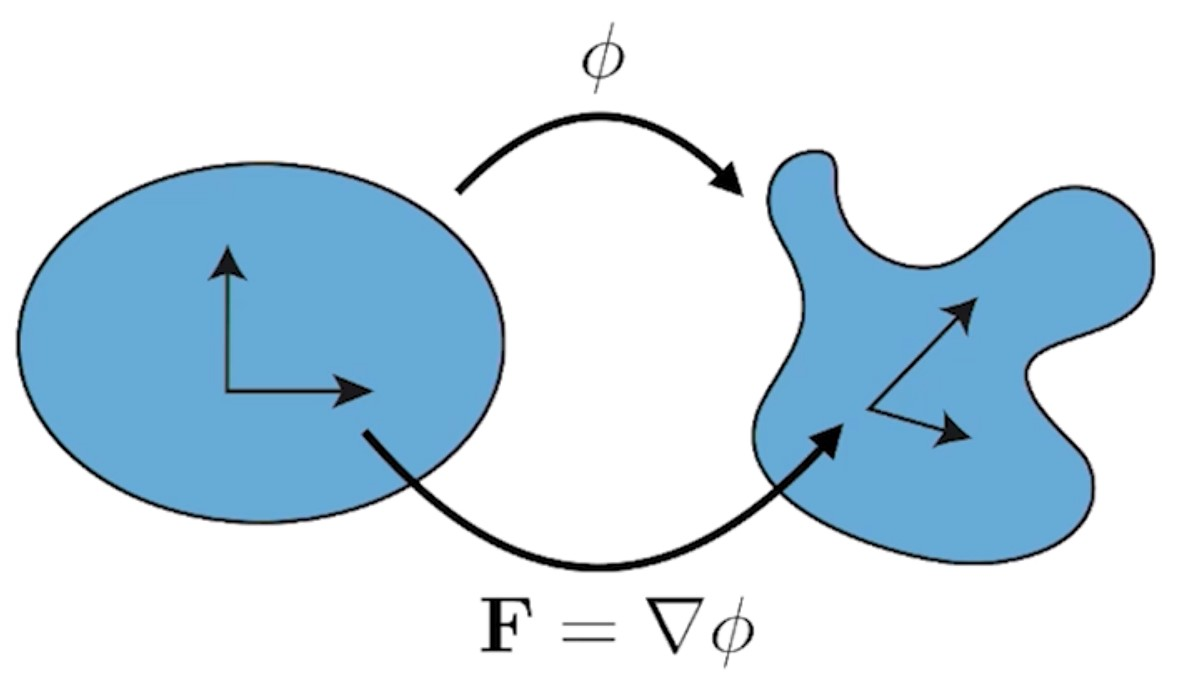
\includegraphics[width=0.5\textwidth]{resources/deformation_map}
	\caption{Deformation Map {\cite{STREAM2018}}}
	\label{fig:deformationmap}
\end{figure}

Each particle $X$ of a body can be characterized by a vector $\mathbf{x}$ containing its coordinates. If the particles undergo a displacement, we can describe their new coordinate vector with 
\[
	\check{\mathbf{x}} = \phi (\mathbf{x}).
\]

When deriving $\phi$, we can calculate the deformation gradient \textbf{F} which serves as a measure of the deformation in the following sense: 
\begin{align*}
&\text{Deformation gradient:} & \mathbf{F}&=\operatorname{\nabla} \phi \\
&\text{Length changes:} & \qquad I_{C}&=\operatorname{tr}\left(\mathbf{F}^{T} \mathbf{F}\right) \\
&\text{Volume changes:} & \qquad J&=\operatorname{det}(\mathbf{F})
\end{align*}

\todoredefined[inline]{
TODO: Explain strain and stress and their meaning for later use in material constants (not explained in paper). Include own image instead of the one here?
}


\subsection{Deformation Gradient}
With the help of the deformation gradient \textbf{F}, we can calculate the change in volume and length of an object during a deformation.
For my needs, I am defining the deformation gradient analogous to the authors of \textit{\acrshort{snh}}:

\begin{equation}\label{eq:deformation_gradient}
\textbf{F} = \left[ \,f_0\, \bigg| \,f_1\, \bigg| \,f_2\, \right] = \begin{bmatrix} f_0 & f_3 & f_6 \\ f_1 & f_4 & f_7 \\ f_2 & f_5 & f_8 \end{bmatrix}.
\end{equation}

\textbf{F} can be factorized in various ways. The next few sections show these factorizations.

\subsubsection{Singular Value Decomposition of F}

Using the SVD theorem shown in Thm.\ref{SVD}, \textbf{F} can be written in the form of

\begin{equation}\label{eq:svd_gradient}
\mathbf{F} = \mathbf{U \Sigma V^\intercal}
\end{equation}

in which $\mathbf{\Sigma}$ stands for
\begin{equation}\label{eq:svd_simga}
\mathbf{\Sigma} = \left[\begin{matrix}  \sigma_0 & 0 & 0 \\ 0 & \sigma_1 & 0 \\ 0 & 0 & \sigma_2 \end{matrix}\right] .
\end{equation}

The $\sigma_i$ denote the singular values of $\mathbf{\Sigma}$.
\textbf{U} and $\mathbf{V^\intercal}$ are both orthogonal matrices that represent the rotation of \textbf{F}. $\Sigma$ on the other hand indicates the scaling of each coordinate $x_i$ by the factor $\sigma_i$.

\todoredefined[inline]{
TODO: Unlike the normal convention, $\mathbf{\Sigma}$ is allowed to have negative entries. --> reflection, maybe add subchapter
\\ Add some examples.
\\ Some more sources:
\\ http://www.continuummechanics.org/deformationgradient.html
}

\subsubsection{Polar Decomposition of the Deformation Gradient}
With the help of Thm.\ref{PD} we can decompose the deformation gradient into the following form
\[
\mathbf{F} = \mathbf{RS}
\]
where \textbf{R} is orthogonal and \textbf{S} is a positive definite symmetric matrix. \textbf{R} symbolises the rotation (with possible reflection) that \textbf{F} undergoes, whereas \textbf{S} contains the scaling along orthogonal directions of \textbf{F}.

\subsubsection{Relative volume change}
A useful information about a deformation is the volume change of the deformed object. It can be calculated by the determinate of \textbf{F}
\[
J = \operatorname{det}(\mathbf{F}).
\]
For a normal deformation, $J$ is a positive value. A determinant of zero would mean that the object is being deformed into a zero volume state e.g. a plane or a point. A negative determinant, on the other hand, indicates an inversion.


\subsubsection{Right Cauchy-Green tensor}

\[
\mathbf{C} = \mathbf{F^\intercal F}
\]

\subsubsection{First right Cauchy -Green invariant}

\[
I_C = \operatorname{\mathbf{C}}
\]

\subsection{Deformation Energy}
In order to get a convincing simulation of high quality, we have to choose an appropriate energy. In the case of modelling deformations on human-like characters an elastic energy needs to be chosen. The key property that makes an energy elastic is that if all the forces that are applied over an object add up to zero, the object must come back into its rest shape.
\\
The energy then has to be minimized in order to get the results we want.

\subsection{Material Constants}
When we look at a deformation of an object, we need to consider the material the object consists of. A material can be very stiff like steel or easily deformable like rubber. In order to measure the deformation of a specific material, we need the \textit{Poisson's Ratio} of said material. The poisson's ratio is a material constant that is defined as 

\begin{equation}\label{eq:poisson}
\sigma = - \frac{\epsilon_{11}}{\epsilon_{22}} \in [-1, 0.5]
\end{equation}

where $\epsilon_{11}$ is the lateral and $\epsilon_{22}$ the axial strain. The range in which $\sigma$ lies in starts at $-1$ and goes up to $0.5$ \cite{PhysRevB.80.132104}. Usually the poisson's ratio of a material is positive. A negative value would mean that the material becomes wider in the cross section when it is stretched. This behaviour is very uncommon in nature. Examples of materials with a negative poisson's ratio are for instance discussed in \textit{Foam structures with a negative Poisson's ratio} \cite{lakes1987foam} or \textit{Advances in negative Poisson's ratio materials} \cite{lakes1993advances}.

Here are some examples of the poisson's ratio of various materials:

\begin{table}[!htbp]
\centering
    \begin{tabular}{ | l | l |}
    \hline
    \textbf{Material} & \textbf{Poisson's ratio} \\ \hline
    C (graphite) & 0.31 \\ \hline
    Sn (metal) & 0.357 \\ \hline
    Cu & 0.355 \\ \hline
    Zn & 0.25 \\ \hline
    Ag & 0.36 \\ \hline
    Au & 0.45 \\ \hline
    Concrete & 0.20–0.37 \\ \hline
    Titanium (dental alloy) & 0.30–0.31 \\ \hline
    Bronze & 0.34 \\ \hline
    18–8 Stainless steel & 0.305 \\ \hline
    Natural rubber & 0.4999 \\ \hline
	B\textsubscript{2}O\textsubscript{3} glass & 0.30 \\ \hline
	GeO\textsubscript{2} glass & 0.20 \\ \hline	
    \end{tabular}
    \caption{Different materials with their poisson's ratio taken from \cite{PhysRevB.80.132104}}
\label{table:1}
\end{table}

In the context of flesh simulations, I am using the poisson's ratio as a characterization for the resistance to volume change of flesh. Biological tissues such as flesh, fat and muscles have one important property: Volume preservation. As a result the poisson's ratio takes on higher values in the range of 0.45 and 0.5 \cite{Smith:2018:SNF:3191713.3180491}.

The calculation of the poisson's ratio defined in Eq. \ref{eq:poisson} is a challenge. Fortunately, we can make use of the \textit{Lamé Parameters}, the two material specific constants $\mu$ and $\lambda$. With the help of these two constants we can transform Eq. \ref{eq:poisson} into the following form:

\begin{equation}\label{eq:poisson_ratio}
\sigma =  \frac{\lambda}{2(\lambda + \mu)}.
\end{equation}

This equation allows to calculate the poisson's ratio much easier. 

\todoredefined[inline]{
TODO: Topic generally covered, maybe adjust the following:
Explain why volume preservation => high poisson's ratio. Explain how to get formula with lamé parameters, explain lamé parameters.
Explain more on negative poisson's value?
\\
Further reading: http://silver.neep.wisc.edu/~lakes/PoissonIntro.html
}



\todoredefined[inline]{
TODO: Add some exaples and visualisations. What exactly is it and what role does it play in a deformation process? Hyperelastic energy, connect with paper.
\\ To include: Piola-Kirchhoff Stress, Cauchy Green invariant, polar decomposition, cauchy green tensor
}





